%%----------------------------------------------------------------------------------------
%	PACKAGES AND THEMES
%----------------------------------------------------------------------------------------
\PassOptionsToPackage{table}{xcolor}
\documentclass[aspectratio=169,xcolor=dvipsnames,svgnames,x11names,fleqn]{beamer}
% \documentclass[aspectratio=169,xcolor=dvipsnames,fleqn]{beamer}

\usetheme{RedVelvet}

\usefonttheme[onlymath]{serif}
\newcommand{\showanswers}{yes}
\usepackage{pifont} % For checkmarks and crosses

\usepackage{setspace}
\usepackage{xspace}
\usepackage{amsmath}
\usepackage{amssymb}
\usepackage{amsfonts}
\usepackage{color}
\usepackage{physics}
% \usepackage{mathbb}
\usepackage{rahul_math}
\usepackage{bigints}

\usepackage[utf8]{inputenc}
\usepackage[ruled,vlined]{algorithm2e}
\usepackage{amsmath}
\usepackage{amsfonts}

\usepackage{graphicx} % Allows including images
\usepackage{booktabs} % Allows the use of \toprule, \midrule and \bottomrule in tables
\usepackage{tikz,pgfplots}
\usepackage{mathtools}
\usepackage{subfigure}
\usetikzlibrary{arrows}
\usepackage{minted}
\definecolor{LightGray}{gray}{0.9}
\definecolor{cream}{rgb}{0.92, 0.9, 0.55}
\definecolor{lightblue}{rgb}{0.68, 0.85, 0.9}


\usepackage{xcolor-material}
\usetikzlibrary{fit}
\usetikzlibrary{matrix}
\tikzset{%
apple/.pic={
    \fill [MaterialBrown] (-1/8,0)  arc (180:120:1 and 3/2) coordinate [pos=3/5] (@)-- ++(1/6,-1/7)  arc (120:180:5/4 and 3/2) -- cycle;
    \fill [MaterialLightGreen500] (0,-9/10)  .. controls ++(180:1/8) and ++(  0:1/4) .. (-1/3,  -1) .. controls ++(180:1/3) and ++(270:1/2) .. (  -1,   0) .. controls ++( 90:1/3) and ++(180:1/3) .. (-1/2, 3/4) .. controls ++(  0:1/8) and ++(135:1/8) .. (   0, 4/7)
    }
    }

\newcommand{\leftdoublequote}{\textcolor{blue}{\scalebox{3}{``}}}

\newcommand{\rightdoublequote}{\textcolor{blue}{\scalebox{3}{''}}}


\usepackage{textcomp}
\usepackage{fontawesome}
\usepackage{tikz,pgfplots}
\usetikzlibrary{shapes.callouts}
\usetikzlibrary{arrows}
\usetikzlibrary{shapes.geometric, positioning}
\usetikzlibrary{matrix,positioning,decorations.pathreplacing,calc}
\usepackage{tikz-dependency}

\pgfplotsset{compat=1.8} % or newest version

\usetikzlibrary{positioning}


\usepackage{bm}
\usepackage{relsize}

\tcbuselibrary{skins, hooks}

\tikzset{basic/.style={draw,fill=MediumBlue!20,text width=1em,text badly centered}}
\tikzset{input/.style={basic,circle}}
\tikzset{weights/.style={basic,rectangle}}
\tikzset{functions/.style={basic,circle,fill=MediumBlue!10}}



\usepackage{listofitems} % for \readlist to create arrays
\tikzstyle{mynode}=[thick,draw=MediumBlue,fill=MediumBlue!20,circle,minimum size=22]


\usepackage{overpic}

%----------------------------------------------------------------------------------------
%	TITLE PAGE
%----------------------------------------------------------------------------------------

\usepackage{tikz-qtree,tikz-qtree-compat}
\usetikzlibrary{tikzmark}
\usetikzlibrary{calc}

\usetikzlibrary{fit}
\tikzset{%
apple/.pic={
    \fill [MaterialBrown] (-1/8,0)  arc (180:120:1 and 3/2) coordinate [pos=3/5] (@)-- ++(1/6,-1/7)  arc (120:180:5/4 and 3/2) -- cycle;
    \fill [MaterialLightGreen500] (0,-9/10)  .. controls ++(180:1/8) and ++(  0:1/4) .. (-1/3,  -1) .. controls ++(180:1/3) and ++(270:1/2) .. (  -1,   0) .. controls ++( 90:1/3) and ++(180:1/3) .. (-1/2, 3/4) .. controls ++(  0:1/8) and ++(135:1/8) .. (   0, 4/7)
}
}
\usepackage{tikz-qtree,tikz-qtree-compat}
\usetikzlibrary{tikzmark}
\usetikzlibrary{calc}

\usetikzlibrary{positioning}
\newcommand{\vect}[1]{\mathbf{#1}}
% Define styles
\tikzset{
    box/.style={
        rectangle,
        draw=black,
        fill=blue!20,
        text width=2.2cm,
        text centered,
        minimum height=0.8cm,
        font=\small
    },
    arrow/.style={
        ->,
        >=Stealth,
        line width=1.5pt,
        draw=black
    }
}


\usepackage{bm}
\usepackage{relsize}



\tikzset{basic/.style={draw,fill=MediumBlue!20,text width=1em,text badly centered}}
\tikzset{input/.style={basic,circle}}
\tikzset{weights/.style={basic,rectangle}}
\tikzset{functions/.style={basic,circle,fill=MediumBlue!10}}
\usetikzlibrary{arrows.meta, bending}
\usetikzlibrary{shapes.geometric, arrows.meta, positioning, fit, backgrounds}

\usepackage{listofitems} % for \readlist to create arrays
\tikzstyle{mynode}=[thick,draw=MediumBlue,fill=MediumBlue!20,circle,minimum size=22]


\newmdenv[
backgroundcolor=androidYellowLight,
linecolor=androidYellow,
linewidth=0.5pt,
roundcorner=10pt,
skipabove=\baselineskip,
skipbelow=\baselineskip
]{MintedFrame}

% Set minted options
\setminted{
fontsize=\footnotesize,
breaklines=true,
autogobble,
linenos,
frame=none
}


\title[CPE 487/587: Deep Learning]{CPE 486/586: Deep Learning for Engineering Applications} % The short title appears at the bottom of every slide, the full title is only on the title page
\subtitle{10 Physics-informed Neural Networks}

\author[Rahul Bhadani] {{\Large \textbf{Rahul Bhadani}}}

\institute[UAH] % Your institution as it will appear on the bottom of every slide, maybe shorthand to save space
{
    Electrical \& Computer Engineering,  The University of Alabama in Huntsville
}
\date

% \titlegraphic{
%    \includegraphics[width=0.4\linewidth]{figures/UAH_primary.png}
% }



\begin{document}

%-------------------------------------------------
\begin{frame}
    \titlepage
\end{frame}

%-------------------------------------------------
\begin{frame}{Outline}
    \backgroundtableofcontents
\end{frame}

%------------------------------------------------
\section{Motivation}
%------------------------------------------------


\begin{frame}{}
    \begin{center}
    \huge \bf \color{DarkBlue}
    Motivation        
\end{center}
\end{frame}

\begin{frame}{Solving a Differential Equation}

\begin{tcolorbox}[    enhanced,
    colback=springBlossom,
    colframe=borderLine,
    arc=0pt, 
    boxrule=0.3pt,
    leftrule=3pt,
    % This creates the orange vertical bar on the left:
    borderline west={5pt}{0pt}{accentOrange}, 
    fontupper=\color{boxBackground},
    pad at break*=0mm,
    top=5pt, bottom=5pt, left=5pt, right=5pt]
    
   Consider a differential equation:
   
   \begin{align*}
   \frac{dx(t)}{dt} = -2x
   \end{align*}

\end{tcolorbox}

How do we solve this Equation?   

\pause 

\vspace{10pt}

Analytically, it is $x = e^{-2t}$ with initial condition $x(0) = 1$.

\pause 

\begin{center}
\Large 

\color{androidRed} But it is usually not analytically possible to solve all kind of differential equations.
\end{center}

\end{frame}

\begin{frame}{Now Data Enters the Picture}

\begin{center}
\color{crimson}
Now, think of a situation when we know $x$ from some measurement of the process and also assume that it follows the differential equation provided earlier.
\end{center}

\pause

\vspace{10pt}

Here, the independent variable is $t$, we know $x$ and we want to find $f$ such that it can give $x$ for any value of $t$.

\pause

\begin{center}
\color{DarkGreen}
\Large
What's the problem then?

\pause 

\vspace{5pt}

\color{DarkRed}
\large 

It may not necessarily be the solution to the differential equation provided earlier!

\end{center}


\end{frame}


\begin{frame}{Differential Equation as Regularizer}

Let's rewrite our differential equation

\begin{tcolorbox}[    enhanced,
    colback=springBlossom,
    colframe=borderLine,
    arc=0pt, 
    boxrule=0.3pt,
    leftrule=3pt,
    % This creates the orange vertical bar on the left:
    borderline west={5pt}{0pt}{accentOrange}, 
    fontupper=\color{boxBackground},
    pad at break*=0mm,
    top=5pt, bottom=5pt, left=5pt, right=5pt]
    
   Consider a differential equation:
   
   \begin{align*}
   \frac{dx(t)}{dt}  + 2x = 0
   \end{align*}

\end{tcolorbox}

But as the real world data will exhibit some error, $x(t)$ might not satisfy the above equation. But if we approximate $x(t)$ using some neural network $u^\theta(x, t)$, we would want

\begin{align*}
\frac{d u^\theta(x, t)}{dt}  + 2 u^\theta(x, t) \leq \varepsilon
\end{align*}
where $\varepsilon$

\end{frame}

\begin{frame}{Differential Equation as Regularizer}

Hence, apart from the training loss, we introduce a physics loss


\begin{tcolorbox}[    enhanced,
    colback=androidRedLight,
    colframe=borderLine,
    arc=0pt, 
    boxrule=0.3pt,
    leftrule=3pt,
    % This creates the orange vertical bar on the left:
    borderline west={5pt}{0pt}{accentOrange}, 
    fontupper=\color{boxBackground},
    pad at break*=0mm,
    top=5pt, bottom=5pt, left=5pt, right=5pt]
    
   Consider a differential equation:
   

$$
\Lcal_{physics} 
$$
which is 

$$
\Lcal_{physics}  = \frac{d u^\theta(x, t)}{dt}  + 2u^\theta(x, t)
$$

for the previous example that we would be looking to minimize.
\end{tcolorbox}

\vspace{10pt}

\begin{center}
This is what we call \textbf{Physics-Informed Deep Learning (PIDL)} or in general \textbf{Physics Informed Machine Learning (PIML)} and the Neural Network used would be called \textbf{Physics-Informed Neural Network (PINN)}.
\end{center}

\end{frame}

\begin{frame}{Updated Loss Function}

\begin{align*}
\Lcal = \lambda_1\Lcal_{data} + \lambda_2 \Lcal_{physics} +  \lambda_3 \Lcal_{IC} + \lambda_4 \Lcal_{BC}
\end{align*}

where $IC$ is for initial conditions and $BC$ is for boundary conditions.

\end{frame}

\begin{frame}{Data + Physics}

\begin{center}
\color{DarkBlue}\Large
Physics governs almost every system we want to model.
\end{center}

\vspace{10pt}
\begin{columns}
  \column{0.5\textwidth}
  \textbf{Classical numerical solvers} (FEM, FDM, FVM):
  \begin{itemize}
    \item Require fine meshes
    \item Scale poorly to high dimensions
    \item Cannot easily solve inverse problems
    \item Need full boundary conditions
  \end{itemize}

  \column{0.5\textwidth}
  \textbf{Pure data-driven ML}:
  \begin{itemize}
    \item Needs enormous labelled data
    \item No physics guarantee
    \item Fails to extrapolate
    \item Black-box predictions
  \end{itemize}
\end{columns}

\vspace{10pt}
\begin{center}
\color{DarkGreen}\Large
\textbf{Can we get the best of both worlds?}
\end{center}


\end{frame}

\begin{frame}{Data Alone is Not Enough}

\begin{columns}
  \column{0.55\textwidth}
  Suppose we fit a neural network $u^\theta(x, t)$ purely on 
  noisy measurements $\{(t_i, \hat{x}_i)\}$.

  \vspace{8pt}
  \textbf{Problems:}
  \begin{itemize}
    \item The network may \textbf{overfit} to noise
    \item \textbf{Extrapolation} outside training region fails
    \item The prediction is \textbf{not guaranteed} to satisfy 
          $\frac{dx}{dt} = -2x$
    \item Different networks with the same data error 
          can give \textbf{physically inconsistent} results
  \end{itemize}

  \column{0.45\textwidth}
  \begin{center}
  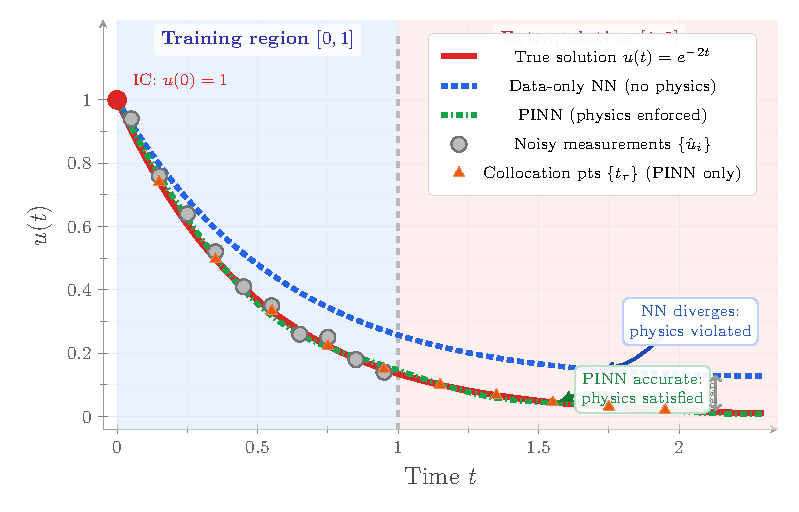
\includegraphics[width=\linewidth]{figures/nn_vs_pinn.pdf}
  \end{center}
  \small
  \textit{Red}: truth \quad \textit{Blue}: data-only NN \quad \textit{Green}: PINN
\end{columns}
\end{frame}

\begin{frame}{The Complete PINN Loss}

We want $u^\theta(x, t)$ to simultaneously:

\begin{enumerate}
  \item \textbf{Fit the data} at measurement points $\{t_i, \hat{x}_i\}$
  \item \textbf{Satisfy the ODE} at collocation points $\{t_r\}$
  \item \textbf{Satisfy the initial condition} $u^\theta(x, 0) = x_0$
\end{enumerate}

\vspace{10pt}
\begin{tcolorbox}[    enhanced,
    colback=androidRedLight,
    colframe=borderLine,
    arc=0pt, 
    boxrule=0.3pt,
    leftrule=3pt,
    % This creates the orange vertical bar on the left:
    borderline west={5pt}{0pt}{accentOrange}, 
    fontupper=\color{boxBackground},
    pad at break*=0mm,
    top=5pt, bottom=5pt, left=5pt, right=5pt]
    \small
$$
\mathcal{L}_\text{total}(\theta) = 
  \underbrace{\lambda_{d}\frac{1}{N_d}\sum_{i=1}^{N_d}\bigl|u^\theta(x, t_i) - \hat{x}_i\bigr|^2}_{\mathcal{L}_\text{data}}
  + \lambda_r\underbrace{\frac{1}{N_r}\sum_{j=1}^{N_r}\Bigl|\frac{du^\theta(x, t_j)}{dt}\Big|_{t_j} + 2u^\theta(x, t_j)\Bigr|^2}_{\mathcal{L}_\text{physics}}
  + \lambda_0\underbrace{\bigl|u^\theta(x, 0) - 1\bigr|^2}_{\mathcal{L}_\text{IC}}
$$
\end{tcolorbox}

\vspace{5pt}
\pause
\begin{center}
\color{DarkBlue}
The physics loss needs \textbf{derivatives of the network output} — these are computed \textit{exactly} via \textbf{automatic differentiation}.
\end{center}
\end{frame}

\begin{frame}{The Complete PINN Loss: General Case}

\footnotesize


\begin{align*}
\mathcal{L}_\text{total}(\theta) & = 
  \underbrace{
    \frac{\lambda_d}{N_d}\sum_{i=1}^{N_d}
    \Bigl|u^\theta(\mathbf{x}_i, t_i) - \hat{u}_i\Bigr|^2
  }_{\mathcal{L}_\text{data}}
  +
  \underbrace{
    \frac{\lambda_r}{N_r}\sum_{j=1}^{N_r}
    \Bigl|\Psi\bigl[u^\theta\bigr](\mathbf{x}_j, t_j) 
    - f(\mathbf{x}_j, t_j)\Bigr|^2
  }_{\mathcal{L}_\text{physics}}
  \\
  &  +
  \underbrace{
    \frac{\lambda_b}{N_b}\sum_{k=1}^{N_b}
    \Bigl|\mathcal{B}\bigl[u^\theta\bigr](\mathbf{x}_k, t_k) 
    - g(\mathbf{x}_k, t_k)\Bigr|^2
  }_{\mathcal{L}_\text{BC}}
  +
  \underbrace{
    \frac{\lambda_0}{N_0}\sum_{m=1}^{N_0}
    \Bigl|u^\theta(\mathbf{x}_m, 0) 
    - u_0(\mathbf{x}_m)\Bigr|^2
  }_{\mathcal{L}_\text{IC}}
\end{align*}

\vspace{10pt}

\footnotesize

\begin{center}
\resizebox{0.7\linewidth}{!}{
\renewcommand{\arraystretch}{1.3}
\begin{tabular}{cll}
\hline
\textbf{Symbol} & \textbf{Meaning} & \textbf{Evaluated on} \\
\hline
$\Psi[\cdot]$ & Differential operator (PDE/ODE) 
  & Interior $\Omega \times (0,T]$ \\
$\mathcal{B}[\cdot]$ & Boundary operator (Dirichlet / Neumann / Robin) 
  & $\partial\Omega \times (0,T]$ \\
$f(\mathbf{x},t)$ & Forcing / source term 
  & \\
$g(\mathbf{x},t)$ & Prescribed boundary value 
  & \\
$u_0(\mathbf{x})$ & Initial condition 
  & $\Omega \times \{t=0\}$ \\
$\lambda_d, \lambda_r, \lambda_b, \lambda_0$ & Loss weights (hyperparameters) 
  & \\
\hline
\end{tabular}
}
\end{center}

\end{frame}

\begin{frame}{Sampling Sets for Each Loss Term}

\begin{center}
\begin{tikzpicture}[scale=0.85]
  % Domain box
  \draw[thick, DarkBlue, fill=blue!5] (0,0) rectangle (6,4);
  \node[DarkBlue] at (3, 3.5) {\small Interior $\Omega$};

  % Interior collocation points (physics loss)
  \foreach \x/\y in {1/1, 1.8/2.5, 2.5/1.4, 3.2/3.0, 
                      4.0/1.8, 4.8/2.8, 5.2/1.2} {
    \filldraw[DarkGreen] (\x,\y) circle (2.5pt);
  }
  \node[DarkGreen] at (5.5, 0.5) {\tiny $\mathbf{x}_j \in \Omega$};

  % Boundary points (BC loss)
  \foreach \x in {0, 1.5, 3, 4.5, 6} {
    \filldraw[androidRed] (\x, 0) circle (2.5pt);
    \filldraw[androidRed] (\x, 4) circle (2.5pt);
  }
  \foreach \y in {0.8, 1.6, 2.4, 3.2} {
    \filldraw[androidRed] (0, \y) circle (2.5pt);
    \filldraw[androidRed] (6, \y) circle (2.5pt);
  }
  \node[androidRed] at (3, -0.35) {\tiny $\mathbf{x}_k \in \partial\Omega$};

  % IC points (bottom time axis)
  \foreach \x in {0.5, 1.5, 2.5, 3.5, 4.5, 5.5} {
    \filldraw[accentOrange] (\x, 0.08) circle (3pt);
  }
\end{tikzpicture}
\end{center}

\vspace{4pt}
\begin{center}
\footnotesize
\textcolor{DarkGreen}{$\bullet$}~Collocation (physics) \quad
\textcolor{androidRed}{$\bullet$}~Boundary (BC) \quad
\textcolor{accentOrange}{$\bullet$}~Initial time $t=0$ (IC) \quad
\textcolor{DarkBlue}{$\bullet$}~Measurement (data, if available)
\end{center}

\vspace{4pt}
\begin{center}
\color{DarkBlue}
\small
None of these sets require a mesh --- points can be placed \textbf{anywhere}, 
including adaptively where the residual is largest.
\end{center}

\end{frame}

\begin{frame}{Two Modes: Forward and Inverse}

\begin{columns}
  \column{0.5\textwidth}
  \begin{tcolorbox}[    enhanced,
    colback=softMint,
    colframe=borderLine,
    sharp corners,
    title=\textbf{Forward Problem},
    arc=0pt, 
    boxrule=0.3pt,
    leftrule=3pt,
    % This creates the orange vertical bar on the left:
    borderline west={5pt}{0pt}{highlightOrange}, 
    fontupper=\color{boxBackground},
    pad at break*=0mm,
    top=5pt, bottom=5pt, left=5pt, right=5pt]
  \textbf{Given:} The PDE + BCs/ICs \\
  \textbf{Find:} The solution $u(x,t)$
  \vspace{5pt}
  \begin{center}
  Physics $\longrightarrow$ Solution
  \end{center}
  \end{tcolorbox}

  \column{0.5\textwidth}
  \begin{tcolorbox}[    enhanced,
    colback=softMint,
    colframe=borderLine,
    sharp corners,
    title=\textbf{Inverse Problem},
    arc=0pt, 
    boxrule=0.3pt,
    rightrule=3pt,
    % This creates the orange vertical bar on the left:
    borderline east={5pt}{0pt}{highlightOrange}, 
    fontupper=\color{boxBackground},
    pad at break*=0mm,
    top=5pt, bottom=5pt, left=5pt, right=5pt]
  \textbf{Given:} Sparse measurements of $u$ \\
  \textbf{Find:} Unknown PDE parameters $\bm\gamma$
  \vspace{5pt}
  \begin{center}
  Measurements $\longrightarrow$ Physics
  \end{center}
  \end{tcolorbox}
\end{columns}

\vspace{10pt}
\pause
\begin{center}
\color{DarkGreen}
\textbf{PINNs handle both in the same framework} \\
\small (just add unknown parameters $\lambda$ as trainable variables)
\end{center}
\end{frame}


\section{Goal}

\begin{frame}
 \sectionpage
 
 \begin{center}
 \bigskip
 
 \large  We want  data-efficient universal function approximators that naturally encode any underlying physical laws as prior information. 
 \end{center}
\end{frame}


\begin{frame}{Differentiable Physics}

We use domain knowledge in the form of model equations.

\begin{itemize}
\item We incorporate discretized version of this model equations into our training process.\end{itemize}



In a supervised settings, we are interested in 

$$
f: X\to Y
$$

Let's assume $\Phi$ be a generic differential equations such that

$$
\Phi: Y \to Z
$$
which encodes a property of the solutions, e.g. some real world behavior we’d like to match. 

  \begin{tcolorbox}[    enhanced,
    colback=softMint,
    colframe=borderLine,
    sharp corners,
    arc=0pt, 
    boxrule=0.4pt,
    leftrule=3pt,
    % This creates the orange vertical bar on the left:
    borderline west={5pt}{0pt}{highlightOrange}, 
    fontupper=\color{boxBackground},
    pad at break*=0mm,
    top=5pt, bottom=5pt, left=5pt, right=5pt]
  In contrast to methods discussed in previous chapters, we use discretized version of $\Phi$, and  and employ it to guide the training of $f$.
  \end{tcolorbox}


\end{frame}


\begin{frame}[fragile]{Example 1: Finding The Inverse Function of Parabola}
\footnotesize


Given $\Phi: x \to x^2$. 

We need to find a function $f \approx \Phi^{-1}$  such that $\Phi(f(x)) = x$ (that is $f(x) \approx \pm \sqrt{x}$. A neural network $f_\theta$ is trained to approximate this. 


\pause

\begin{columns}[c]

\column{0.5\linewidth}

Data is $
 \Dcal \{(x^{(i)}, y^{(i)})\}_{i=1}^N
$ where $y^{(i)} = \pm\sqrt{x}^{(i)}$.


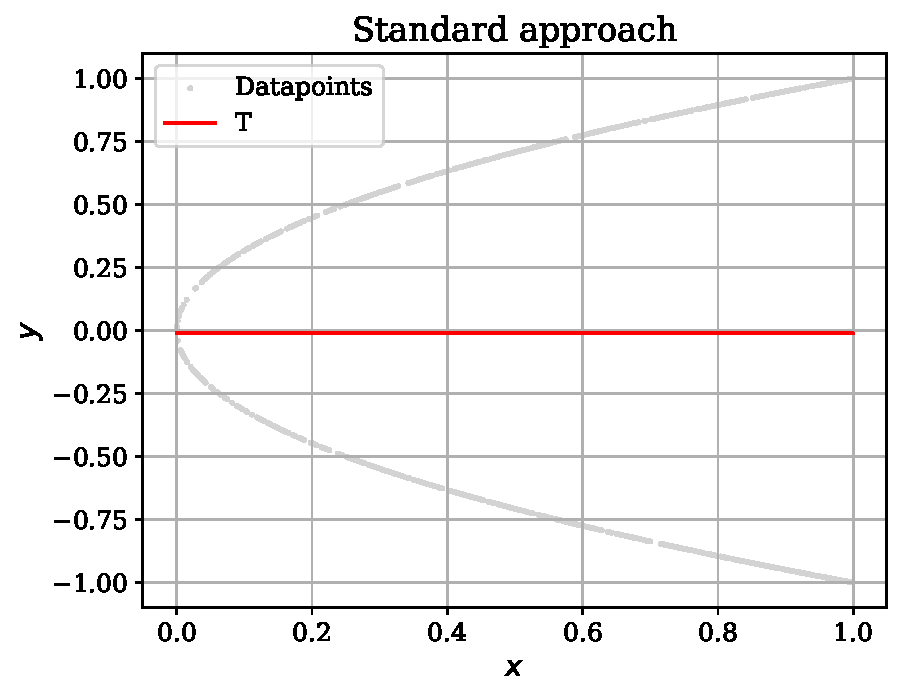
\includegraphics[width=0.7\linewidth]{figures/parabola_supervised_nn.pdf}

Loss: $\frac{1}{n}\sum_{i=1}^N ( f_\theta(x^{(i)}) - y^{(i)} )^2$

\column{0.5\linewidth}

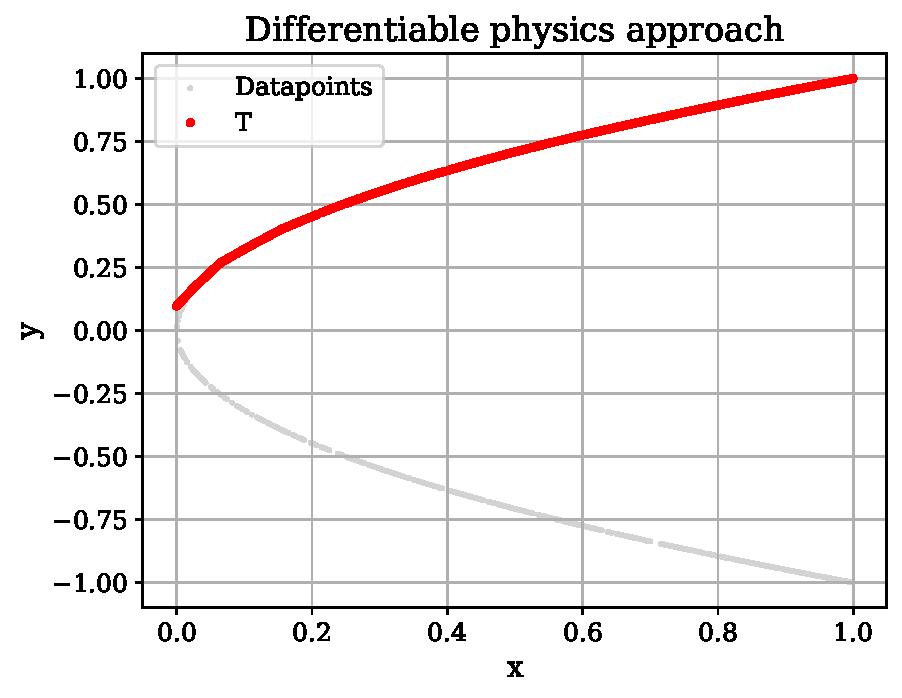
\includegraphics[width=0.7\linewidth]{figures/parabola_physics_nn.pdf}

Loss: $\frac{1}{n}\sum_{i=1}^N ( \Phi(f_\theta(x^{(i)})) - x^{(i)} )^2$.


  \begin{tcolorbox}[    enhanced,
    colback=softMint,
    colframe=borderLine,
    sharp corners,
    arc=0pt, 
    boxrule=0.4pt,
    leftrule=3pt,
    % This creates the orange vertical bar on the left:
    borderline west={5pt}{0pt}{highlightOrange}, 
    fontupper=\color{boxBackground},
    pad at break*=0mm,
    top=2pt, bottom=2pt, left=5pt, right=5pt]
Here, no $y^{(i)}$ is used, but only the input $x^{(i)}$ and known forward operator $\Phi$.
\end{tcolorbox}


\end{columns}

\end{frame}

\begin{frame}[fragile]{Backpropagation in Physics Loss}

\footnotesize


\begin{columns}

\column{0.4\linewidth}

For the physics loss, backprop through $\Phi$ gives 

$$
\pdv{\Lcal_{phys}}{f_\theta(x^{(i)})} = 4 f_\theta (x^{(i)})(f_\theta(x^{(i)})^2  - x^{(i)})
$$

Its derivative vanishes at $f_\theta(x^{(i)}) = 0$, regardless of $x^{(i)}$. Hence, the zero function is a saddle point of the physics loss that doesn't affect the supervised loss.

\column{0.6\linewidth}


\resizebox{\linewidth}{!}{
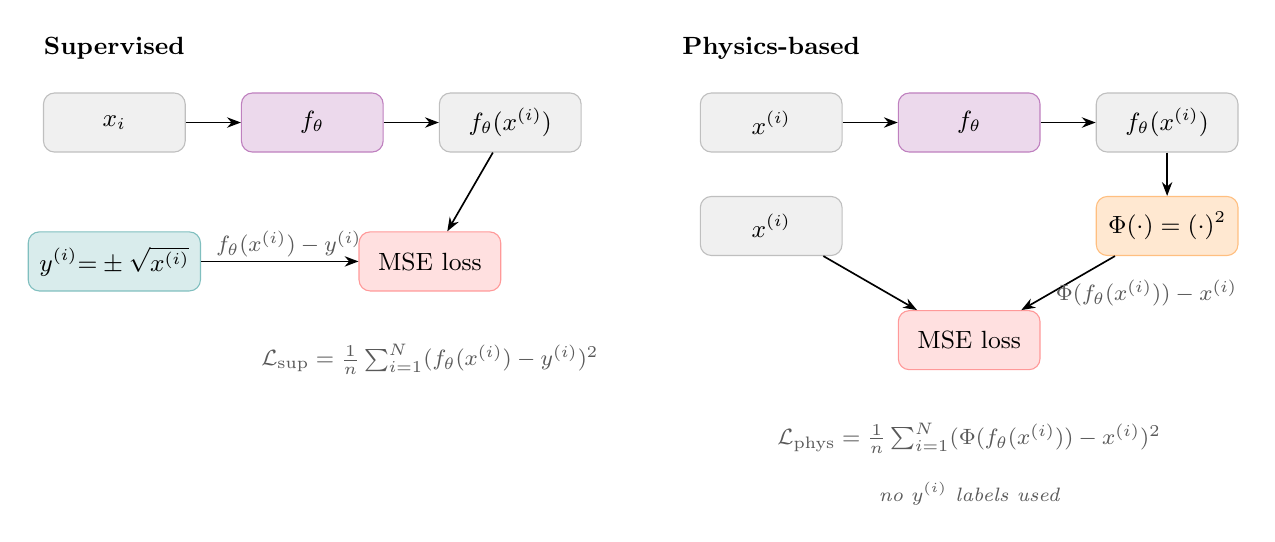
\begin{tikzpicture}[
  node distance = 0.55cm and 0.7cm,
  box/.style = {
    draw, rounded corners=4pt, minimum width=1.8cm, minimum height=0.75cm,
    font=\small, align=center, inner sep=4pt
  },
  gray box/.style  = {box, fill=gray!12,  draw=gray!50},
  purple box/.style= {box, fill=violet!15, draw=violet!50},
  teal box/.style  = {box, fill=teal!15,  draw=teal!50},
  amber box/.style = {box, fill=orange!18, draw=orange!50},
  coral box/.style = {box, fill=red!12,   draw=red!40},
  arr/.style = {-{Stealth[length=5pt]}, semithick},
  label/.style = {font=\footnotesize, text=gray!70!black},
]

\node[gray box]   (xi-s)  {$x_i$};
\node[purple box] (f-s)   [right=of xi-s]  {$f_\theta$};
\node[gray box]   (fx-s)  [right=of f-s]   {$f_\theta(x^{(i)})$};
\node[teal box]   (yi)    [below=1.0cm of xi-s]  {$y^{(i)} {=} \pm\sqrt{x^{(i)}}$};
\node[coral box]  (mse-s) [right=2.0cm of yi]    {MSE loss};

\draw[arr] (xi-s) -- (f-s);
\draw[arr] (f-s)  -- (fx-s);
\draw[arr] (fx-s) -- (mse-s);
\draw[arr] (yi)   -- (mse-s);

\node[label, above right=-2pt and 2pt of yi.east] {$f_\theta(x^{(i)}) - y^{(i)}$};

\node[label, below=0.55cm of mse-s, align=center]
  {$\mathcal{L}_{\mathrm{sup}} = \frac{1}{n}\sum_{i=1}^N ( f_\theta(x^{(i)}) - y^{(i)} )^2$};

\node[font=\small\bfseries, above=0.3cm of xi-s] {Supervised};

\coordinate (div-top) at ($(fx-s.east)!0.5!(f-s.east) + (1.1cm, 1.0cm)$);
\coordinate (div-bot) at ($(div-top) + (0,-4.2cm)$);


\node[gray box]   (xi-p)  [right=1.5cm of fx-s]  {$x^{(i)}$};
\node[purple box] (f-p)   [right=of xi-p]         {$f_\theta$};
\node[gray box]   (fx-p)  [right=of f-p]          {$f_\theta(x^{(i)})$};
\node[amber box]  (Phi)   [below=of fx-p]         {$\Phi(\cdot)=(\cdot)^2$};
\node[coral box]  (mse-p) [below=2.0cm of f-p]          {MSE loss};
\node[gray box]   (xi-p2) [below=of xi-p]         {$x^{(i)}$};

\draw[arr] (xi-p)  -- (f-p);
\draw[arr] (f-p)   -- (fx-p);
\draw[arr] (fx-p)  -- (Phi);
\draw[arr] (Phi)   -- (mse-p);
\draw[arr] (xi-p2) -- (mse-p);

\node[label, above right=-2pt and 2pt of mse-p.north east, align=left]
  {$\Phi(f_\theta(x^{(i)})) - x^{(i)}$};

\node[label, below=0.55cm of mse-p, align=center]
  {$\mathcal{L}_{\mathrm{phys}} =\frac{1}{n}\sum_{i=1}^N ( \Phi(f_\theta(x^{(i)})) - x^{(i)} )^2$};

\node[label, below=1.3cm of mse-p, align=center, font=\scriptsize\itshape]
  {no $y^{(i)}$ labels used};

\node[font=\small\bfseries, above=0.3cm of xi-p] {Physics-based};

\end{tikzpicture}
}


\end{columns}

\end{frame}

\begin{frame}{}

\Large

\begin{center}
{

\color{algoColorKey}

Clearly, it didn't handle  the \textbf{bifurcation}.

\vspace{10pt}


\color{pinnColor}

Can we do better?

}

\pause 

\vspace{10pt}

We can learn the full distribution of the posterior.

\pause 

\vspace{10pt}

\color{trueColor}

Do you remember \textbf{Flow Matching}?



\end{center}

\end{frame}


\begin{frame}{Flow  Matching for Inverse Function of Parabola}

Assuming, normalized time, i.e. $t \sim \Ucal[0, 1]$.

{\vspace{3pt}\color{peachFuzz}\hrule\vspace{3pt}}

Recall, data is $ \Dcal \{\xbf^{(i)} \equiv (x^{(i)}, y^{(i)})\}_{i=1}^N $ where $y^{(i)} = \pm\sqrt{x^{(i)}}$.

{\vspace{3pt}\color{peachFuzz}\hrule\vspace{3pt}}

We define  $\xbf \sim \Ncal(0, \Ibf_2)$. Initial condition $\xbf^{(i)}_0[0] = x^{(i)}$ (we fix x-coordinate noise).

{\vspace{3pt}\color{peachFuzz}\hrule\vspace{3pt}}

For every sample index $i$, the end point should be $\xbf^{(i)}_1 = (x^{(i)}, y^{(i)})^\top$.


{\vspace{3pt}\color{peachFuzz}\classicRule\vspace{3pt}}


As we need to define a probability path $p_t$, but as we understand the $p_t$ being marginal is difficult to compute.

\vspace{5pt}
Conditional interpolant can help in this case. We fix a specific pair and define a deterministic path between them, such as,

\begin{align*}
\xbf_t \big|_{(\xbf_0, \xbf_1)} = (1 - t)\xbf_0  + t \xbf_1
\end{align*}

\vspace{10pt}

\textbf{But remember that the interpolant doesn't have to be linear.}
\end{frame}


\begin{frame}{Flow  Matching for Inverse Function of Parabola}

The marginal interpolant $p_t(\xbf)$ is recovered by averaging over all pairs:

  \begin{tcolorbox}[    enhanced,
    colback=softMint,
    colframe=borderLine,
    sharp corners,
    arc=0pt, 
    boxrule=0.4pt,
    leftrule=3pt,
    % This creates the orange vertical bar on the left:
    borderline west={5pt}{0pt}{highlightOrange}, 
    fontupper=\color{boxBackground},
    pad at break*=0mm,
    top=1pt, bottom=2pt, left=5pt, right=5pt]
\begin{align*}
p_t(\xbf) = \int p_t(\xbf_t \big|_{(\xbf_0, \xbf_1)}) q(\xbf_0)p_{data}(\xbf_1) d\xbf_0 d\xbf_1
\end{align*}
\end{tcolorbox}

And, we have target conditional vector field as $u_t = \frac{dx_t}{dt}$, which is always deterministic, that is $x_1 - x_0$ (only applicable for linear interpolant, for non-linear interpolant, you will see $t$ in RHS of $u_t$).

\vspace{5pt}

\fleuronRule

\vspace{5pt}

We can define a neural network $v_\theta(\xbf_t, t)$ that will regress $u_t$ with Flow Matching Loss function:

\begin{align*}
\Lcal_{FM}(\theta) = \frac{1}{n}\sum_{i=1}^N ||  v_\theta( \xbf_t^{(i)}, t^{(i)}) - u_t^{(i)}||^2
\end{align*}


\end{frame}

\begin{frame}{Flow  Matching for Inverse Function of Parabola}

At the inference time (prediction with the trained model), given $\xbf_0 = (x^{(i)},z )^\top$ with $z \sim \Ncal(0, 1)$, the integrate the learned ODE model with step size $\Delta t = \frac{1}{T}$:

\begin{align*}
\xbf_{t_{k+1}}^{(i)} = \xbf_{t_{k}}^{(i)}  + \Delta t v_\theta (  \xbf_{t_{k}}^{(i)}, t_k)
\end{align*}

and then reimpose the x-conditioning at every step: $\xbf_{t_{k+1}}^{(i)}[0] \leftarrow x^{(i)}$ and we get the second coordinate of the final state 

\begin{align*}
\xbf_{t_1}^{(i)}[1] \sim p(y|x^{(i)})
\end{align*}

\end{frame}


\begin{frame}{Flow  Matching for Inverse Function of Parabola}

\resizebox{0.7\linewidth}{!}
{
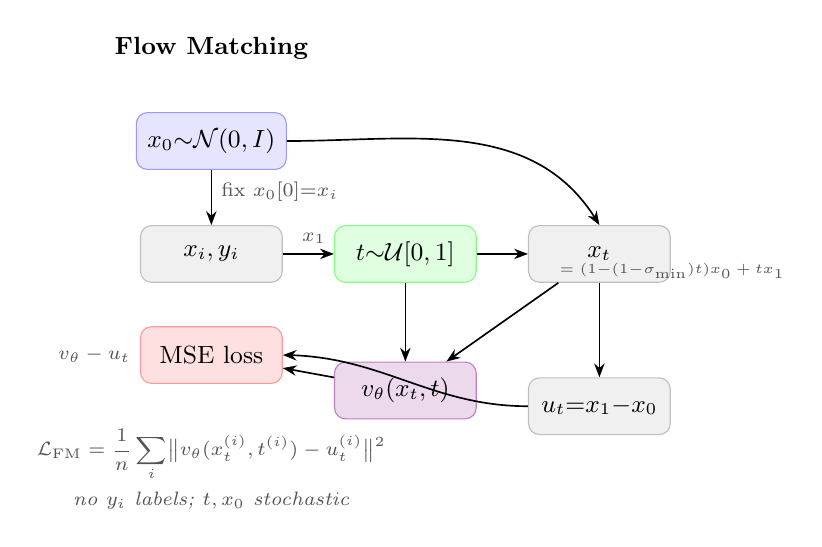
\begin{tikzpicture}[
  node distance = 0.55cm and 0.65cm,
  box/.style = {
    draw, rounded corners=4pt, minimum width=1.8cm, minimum height=0.72cm,
    font=\small, align=center, inner sep=4pt
  },
  gray box/.style   = {box, fill=gray!12,   draw=gray!50},
  purple box/.style = {box, fill=violet!15,  draw=violet!50},
  teal box/.style   = {box, fill=teal!15,   draw=teal!50},
  amber box/.style  = {box, fill=orange!18,  draw=orange!50},
  coral box/.style  = {box, fill=red!12,    draw=red!40},
  blue box/.style   = {box, fill=blue!10,   draw=blue!40},
  green box/.style  = {box, fill=green!12,  draw=green!50},
  arr/.style   = {-{Stealth[length=5pt]}, semithick},
  label/.style = {font=\scriptsize, text=gray!65!black},
]

\node[gray box]   (xi-fm)  []  {$x_i, y_i$};
\node[blue box]   (x0)     [above=0.7cm of xi-fm] {$x_0{\sim}\mathcal{N}(0,I)$};
\node[green box]  (t-node) [right=of xi-fm]        {$t{\sim}\mathcal{U}[0,1]$};

% Interpolant node
\node[gray box]   (xt)  [right=of t-node]  {$x_t$};
\node[gray box]   (ut)  [below=1.2cm of xt]      {$u_t{=}x_1{-}x_0$};

% velocity net
\node[purple box] (vnet)  [below=1.0cm of t-node] {$v_\theta(x_t,t)$};

% loss
\node[coral box]  (mse-fm) [below=of xi-fm]  {MSE loss};

% arrows
\draw[arr] (xi-fm)  -- node[above, label, xshift=2pt]{$x_1$} (t-node);
\draw[arr] (x0)     -- node[right, label, yshift=2pt]{fix $x_0[0]{=}x_i$} (xi-fm);
\draw[arr] (t-node) -- (xt);
\draw[arr] (x0.east) to[out=0,in=120] (xt.north);
\draw[arr] (xt) -- (ut);
\draw[arr] (xt)  -- (vnet);
\draw[arr] (t-node) -- (vnet);
\draw[arr] (vnet) -- (mse-fm);
\draw[arr] (ut.west)  to[out=180,in=0] (mse-fm.east);

\node[label, left=0pt of mse-fm.west, yshift=0pt]
  {$v_\theta - u_t$};

% interpolant label
\node[label, above right=-2pt and 8pt of xt.south west, align=left, font=\tiny]
  {$= (1{-}(1{-}\sigma_{\min})t)x_0+tx_1$};

\node[label, below=0.45cm of mse-fm, align=center]
  {$\mathcal{L}_{\mathrm{FM}} =
    \dfrac{1}{n}\displaystyle\sum_{i}
    \bigl\|v_\theta(x_t^{(i)}, t^{(i)}) - u_t^{(i)}\bigr\|^2$};

\node[label, below=1.25cm of mse-fm, font=\scriptsize\itshape]
  {no $y_i$ labels; $t,x_0$ stochastic};

\node[font=\small\bfseries, above=0.55cm of x0] {Flow Matching};

\end{tikzpicture}
}

\end{frame}

\begin{frame}{Flow  Matching for Inverse Function of Parabola}

Caveats about Flow Matching:

\begin{itemize}
\item Flow Matching is \textbf{not} PINN.
\item Physics get introduced in data construction $y^{(i)} = \pm \sqrt{x^{(i)}}$ but FM never sees $\Phi$.
\item It learns conditional distributipn $p(y|x)$.
\item In the case of FM, the parabola $y^2 = x$ is the \textbf{support manifold} of that distribution, but no operator passed to the loss.
\end{itemize}

\end{frame}

\begin{frame}{Flow Matching for Inverse Function of Parabola}

\begin{center}

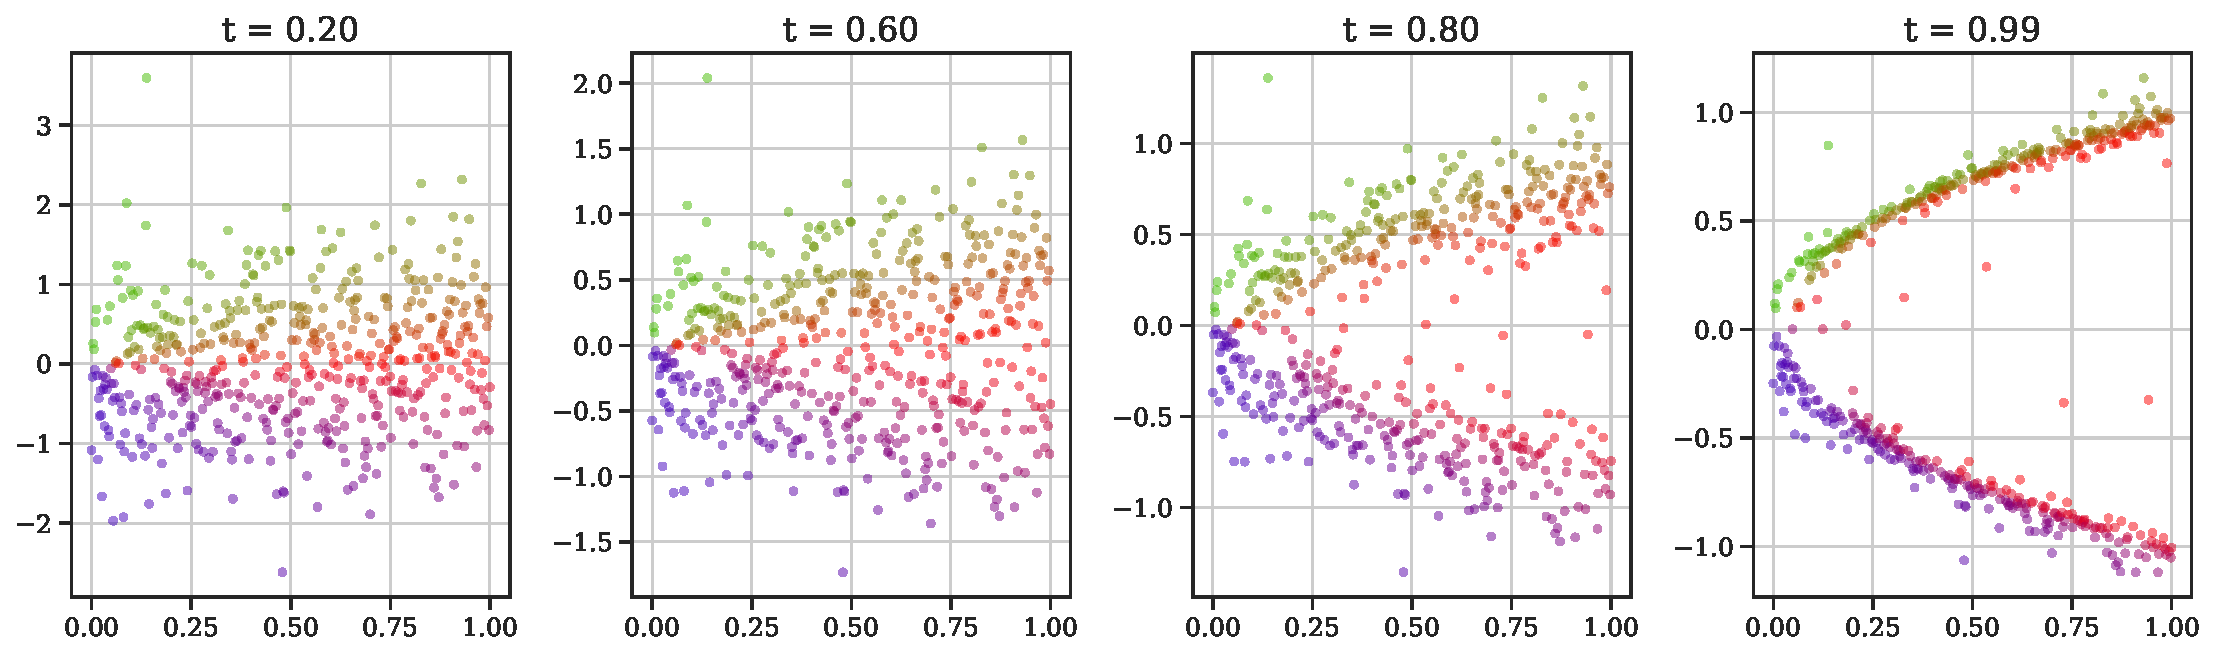
\includegraphics[width=0.8\linewidth]{figures/FM_probability_path_evo.pdf}



\begin{columns}

\column{0.5\linewidth}

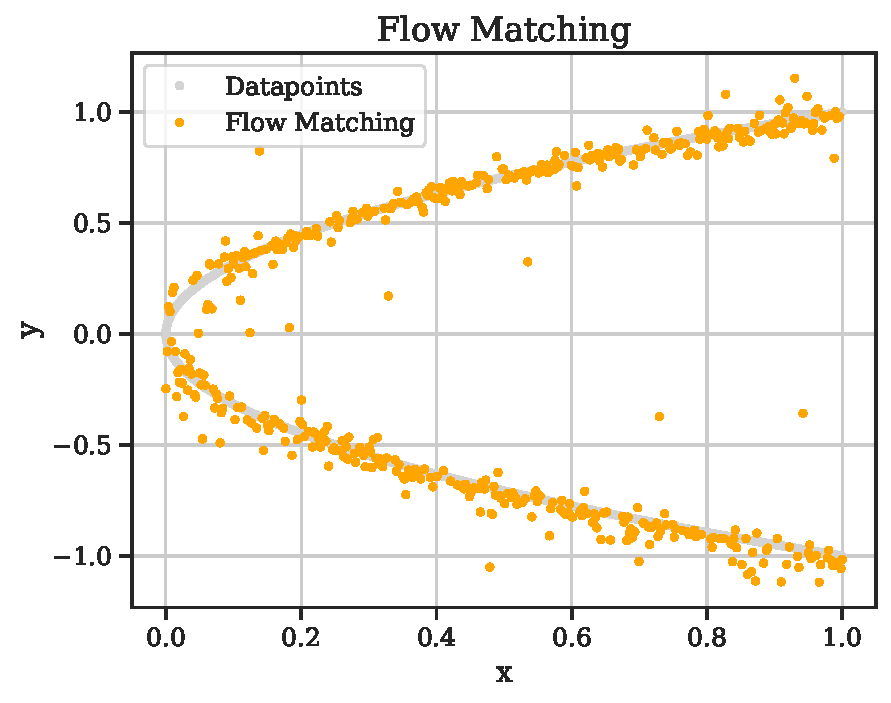
\includegraphics[width=0.6\linewidth]{figures/FM_training.pdf}

\column{0.5\linewidth}

\scriptsize

Clearly, Flow Matching provides an approximate solution, although allows to take into account Bifurcation but makes mistakes as well. 

\textbf{FM is not PINN. }

\end{columns}



\end{center}



\end{frame}


\begin{frame}{References}

\scriptsize

\begin{itemize}

\item Physics-informed machine learning \url{https://doi.org/10.1038/s42254-021-00314-5}

\item Physics Informed Deep Learning (Part I): Data-driven Solutions of Nonlinear Partial Differential Equations \url{https://arxiv.org/abs/1711.10561}

\item Physics Informed Deep Learning (Part II): Data-driven Discovery of Nonlinear Partial Differential Equations \url{https://arxiv.org/abs/1711.10566}

\item Thuerey, Nils, Philipp Holl, Maximilian Mueller, Patrick Schnell, Felix Trost, and Kiwon Um. "Physics-based deep learning." arXiv preprint arXiv:2109.05237 (2021). \url{https://arxiv.org/abs/2109.05237}

\item Physics-informed neural networks: A deep learning framework for solving forward and inverse problems involving nonlinear partial differential equations
Author links open overlay panel \url{https://doi.org/10.1016/j.jcp.2018.10.045}


\item \url{https://github.com/maziarraissi/PINNs}

\item \url{https://github.com/prateekbhustali/Physics-Informed-Neural-Networks}

\item \url{https://github.com/nguyenkhoa0209/pinns_tutorial}

\item \url{https://annien094.github.io/PINNs-tutorial-MICCAI-2024/}

\item Physics-informed neural networks for PDE problems: a comprehensive review \url{https://doi.org/10.1023/a:1012784129883}

\item A hands-on introduction to Physics-Informed Neural Networks for solving partial differential equations with benchmark tests taken from astrophysics and plasma physics \url{https://arxiv.org/pdf/2403.00599}

\end{itemize}

\end{frame}



\end{document}